\chapter{従来手法}

  本研究のベースとなる岡田らの研究(以後,従来手法と呼ぶ)について述べる.従来手法は,引き紐を用いたルールベース制御器による行動を模倣学習し,同様の行動を画像を用いて行う手法である.この手法は,学習フェーズと追従フェーズに分かれている.

\label{chap:trajectory}
%
%!TEX root = ../thesis.tex

\section{学習フェーズ}

  学習フェーズで使用するルールベース制御器を\figref{Fig:okada_rule-based_contoroller}に示す.ルールベース制御器は,引き紐に取り付けられたポテンショメータからのリンクの角度を入力とし,ルールに従いロボットは行動を選択する.ルールベース制御器からの出力を\tabref{tab:actions_control_parameters}に示す.なお,並進速度は0.1 \,[m/s]で一定である.

  \begin{figure}[h]
    \centering
    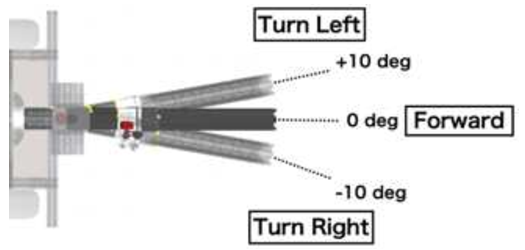
\includegraphics[keepaspectratio, scale=1.1] {images/pdf/okada_rule-based_contoroller}
    \caption[Action according to angles of the joint]{Action according to angles of the joint (source: \cite{okada})}
    \label{Fig:okada_rule-based_contoroller}
  \end{figure}

  \vspace{1cm}

  \begin{table}[ht]
    \caption{The control rule and action parameters}
    \label{tab:actions_control_parameters}
    \centering
    \begin{tabular}{cccc}
    \hline
    Action & Control rule & Linear velocity & Angular velocity \\ 
    \hline
    \hline
    Turn Left & $\theta_{\mathrm{yaw}} > 10 \, \mathrm{deg}$ & 0.1 \,m/s & 0.2 \,rad/s \\ 
    Forward & $-10 \, \mathrm{deg} < \theta_{\mathrm{yaw}} < 10 \, \mathrm{deg}$ & 0.1 \,m/s & 0 \,rad/s \\ 
    Turn Right & $\theta_{\mathrm{yaw}} < -10 \, \mathrm{deg}$ & 0.1 \,m/s & -0.2 \,rad/s \\ 
    \hline
    \end{tabular}
    \end{table}
  
\newpage
%!TEX root = ../thesis.tex

\section{追従フェーズ}

  追従フェーズでは,学習フェーズで学習したモデルを活用し,\figref{Fig:okada_route}に示す経路(学習フェーズと同じ経路)を使用してテストを行う.この際,引き紐は不要であり,代わりに深層学習器に画像が入力され,その出力がロボットの行動となる.つまり,学習フェーズで利用された引き紐によるルールベース制御器の出力ではなく,カメラ画像に基づく深層学習器の出力がロボットの行動になる.

  \begin{figure}[h]
    \centering
    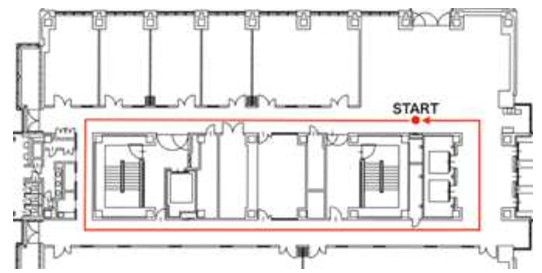
\includegraphics[keepaspectratio, scale=0.70] {images/pdf/okada_route}
    \caption[Target trajectory that the operator walks]{Target trajectory that the operator walks (source: \cite{okada})}
    \label{Fig:okada_route}
  \end{figure}

\newpage
%!TEX root = ../thesis.tex

\section{ネットワークの構造}

  ネットワークを\figref{Fig:okada_network}に示す.これは,深層学習フレームワークであるChainer\cite{chainer}を使用し,CNNをベースとしている.具体的には,入力層,畳み込み層3,全結合層2,出力層の7層で構成されている.深層学習器は,縮小された画像と選択された行動を0.6秒周期で収集して学習する.これに使用されたハイパーパラメータを\tabref{tab:Parameters of network configured with chainer}に示す.

  \begin{figure}[h]
    \centering
    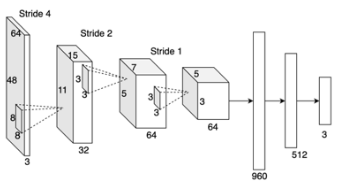
\includegraphics[keepaspectratio, scale=0.70] {images/okada_network.png}
    \caption[Structure of the network]{Structure of the network (source: \cite{okada})}
    \label{Fig:okada_network}
  \end{figure}

  \begin{table}[hbtp]
    \caption{Parameters of network configured with chainer}
    \label{tab:Parameters of network configured with chainer}
    \centering
    \begin{tabular}{cc}
      \hline
      Input data & Image(64x48 pixels, RGB channels) \\
      Optimizer & Adam($alpha = 0.001, beta1 = 0.9, beta2 =  0.999, eps = 1e^{-2}$)\\
      Loss function & Softmax-cross-entropy\\
      Output data & Action (Forward, Turn Left, Turn Right)\\
      \hline
    \end{tabular}
  \end{table}

\newpage


%
